%%%%%%%%%%%%%%%%%%%%%%%%%%%%%%%%%%%%%%%%%
% Short Sectioned Assignment LaTeX Template Version 1.0 (5/5/12)
% This template has been downloaded from: http://www.LaTeXTemplates.com
% Original author:  Frits Wenneker (http://www.howtotex.com)
% License: CC BY-NC-SA 3.0 (http://creativecommons.org/licenses/by-nc-sa/3.0/)
%%%%%%%%%%%%%%%%%%%%%%%%%%%%%%%%%%%%%%%%%

%----------------------------------------------------------------------------------------
%	PACKAGES AND OTHER DOCUMENT CONFIGURATIONS
%----------------------------------------------------------------------------------------

\documentclass[paper=a4, fontsize=11pt]{scrartcl} % A4 paper and 11pt font size

% ---- Entrada y salida de texto -----

\usepackage[T1]{fontenc} % Use 8-bit encoding that has 256 glyphs
\usepackage[utf8]{inputenc}
%\usepackage{fourier} % Use the Adobe Utopia font for the document - comment this line to return to the LaTeX default

% ---- Idioma --------

\usepackage[spanish, es-tabla]{babel} % Selecciona el español para palabras introducidas automáticamente, p.ej. "septiembre" en la fecha y especifica que se use la palabra Tabla en vez de Cuadro

% ---- Otros paquetes ----

\usepackage{url} % ,href} %para incluir URLs e hipervínculos dentro del texto (aunque hay que instalar href)
\usepackage{amsmath,amsfonts,amsthm} % Math packages
%\usepackage{graphics,graphicx, floatrow} %para incluir imágenes y notas en las imágenes
\usepackage{graphics,graphicx, float} %para incluir imágenes y colocarlas

% Para hacer tablas comlejas
%\usepackage{multirow}
%\usepackage{threeparttable}

%\usepackage{sectsty} % Allows customizing section commands
%\allsectionsfont{\centering \normalfont\scshape} % Make all sections centered, the default font and small caps

\usepackage{fancyhdr} % Custom headers and footers
\pagestyle{fancyplain} % Makes all pages in the document conform to the custom headers and footers
\fancyhead{} % No page header - if you want one, create it in the same way as the footers below
\fancyfoot[L]{} % Empty left footer
\fancyfoot[C]{} % Empty center footer
\fancyfoot[R]{} % Page numbering for right footer
\renewcommand{\headrulewidth}{0pt} % Remove header underlines
\renewcommand{\footrulewidth}{0pt} % Remove footer underlines
\setlength{\headheight}{13.6pt} % Customize the height of the header

\numberwithin{equation}{section} % Number equations within sections (i.e. 1.1, 1.2, 2.1, 2.2 instead of 1, 2, 3, 4)
\numberwithin{figure}{section} % Number figures within sections (i.e. 1.1, 1.2, 2.1, 2.2 instead of 1, 2, 3, 4)
\numberwithin{table}{section} % Number tables within sections (i.e. 1.1, 1.2, 2.1, 2.2 instead of 1, 2, 3, 4)

\setlength\parindent{0pt} % Removes all indentation from paragraphs - comment this line for an assignment with lots of text

\newcommand{\horrule}[1]{\rule{\linewidth}{#1}} % Create horizontal rule command with 1 argument of height


\usepackage{hyperref}
\usepackage{listings}
\usepackage{xcolor}
\usepackage{caption}
\usepackage{subcaption}
\usepackage{lmodern}
\usepackage{graphicx}
\usepackage{biblatex}
\usepackage{array}
\usepackage{wrapfig}

\definecolor{codegreen}{rgb}{0,0.6,0}
\definecolor{codegray}{rgb}{0.5,0.5,0.5}
\definecolor{codepurple}{rgb}{0.58,0,0.82}
\definecolor{backcolour}{rgb}{0.95,0.95,0.92}
\usepackage[margin=0.7in]{geometry}

\newcolumntype{C}[1]{>{\centering\arraybackslash}p{#1}}
\newcolumntype{L}[1]{>{\raggedright\arraybackslash}p{#1}}
\newcolumntype{R}[1]{>{\raggedleft\arraybackslash}p{#1}}

\lstdefinestyle{mystyle}{
    backgroundcolor=\color{backcolour},   
    commentstyle=\color{codegreen},
    keywordstyle=\color{magenta},
    numberstyle=\tiny\color{codegray},
    stringstyle=\color{codepurple},
    basicstyle=\ttfamily\footnotesize,
    breakatwhitespace=false,         
    breaklines=true,                 
    captionpos=b,                    
    keepspaces=true,                 
    numbers=left,                    
    numbersep=5pt,                  
    showspaces=false,                
    showstringspaces=false,
    showtabs=false,                  
    tabsize=2
}


\title{	
\normalfont \normalsize 
\textsc{\textbf{Metaheurística grupo 2 (2021-2022)} \\ Grado en Ingeniería Informática \\ Universidad de Granada} \\ [25pt] % Your university, school and/or department name(s)
\horrule{0.5pt} \\[0.4cm] % Thin top horizontal rule
\huge Práctica 2 \\
Mínima dispersión diferencial \\ % The assignment title
\horrule{2pt} \\[0.5cm] % Thick bottom horizontal rule
}

\author{José María Ramírez González\\\href{mailto:jmramirez@correo.ugr.es}{jmramirez@correo.ugr.es}} % Nombre y apellidos

\date{\normalsize\today} % Incluye la fecha actual

\begin{document}

\maketitle % Muestra el Título

\newpage %inserta un salto de página

\tableofcontents % para generar el índice de contenidos

\newpage

\section{Descripción del problema}

El problema escogido es el conocido como \textit{mínima dispersión diferencial} o \textit{minimun differential dispersion} en inglés.

En este problema se intenta minimizar la dispersión entre un subconjunto $M$ de elementos de un conjunto $C$. Es un problema \textbf{NP-completo}, por lo que resulta inviable resolverlo de manera óptima en un tiempo decente en casos donde $|C|$ o $|M|$ sean grandes.

Nuestro objetivo es encontrar $M \subset C$, y se nos proporcionarán varios casos, cada uno con un $C$ y un $m =|M|$.
En cada caso nos dan, además, la distancia de un elemento al resto de ellos, tal que podamos calcular el \textit{$\Delta$-value} de cada elemento como $\displaystyle \Delta \text{-value}_i = \sum_{j \in M}d_{ij}\quad \forall \, i \in M$, donde $d_{ij}$ es la distancia del elemento $i$ al elemento $j$.

Para calcular la dispersión, realizamos el siguiente cálculo $disp = max(\Delta\text{-value})-min(\Delta\text{-value})$. Esa sería la dispersión asociada a una posible solución $M$, el máximo de sus $\Delta$-values menos el mínimo de ellos. Así pues, nuestra función a minimizar es esa.

Es importante destacar que la dispersión de cada conjunto solución $M$ depende de cada uno de los elementos $w \in M$ y que, cambiando tan solo uno de ellos, esta puede cambiar radicalmente.

\section{Elementos comunes empleados en la resolución del problema}
Para resolver este problema, hemos implementado los siguientes algoritmos:
\begin{itemize}
\item Un algoritmo \textbf{Greedy}.
\item Un algoritmo de \textbf{Búsqueda local}.
\item Un algoritmo \textbf{Genético Generacional (AGG)}.
\item Un algoritmo \textbf{Genético Estacional (AGE)}.
\item Un algoritmo \textbf{Memético (AM)}.
\end{itemize}

El código de los algoritmos de la práctica anterior, \textit{greedy} y \textit{búsqueda local} estará comentado, ya que no es relevante para lo que se remite a esta práctica, no obstante, podremos descomentarlo\footnote{Líneas 173-184, 186-251, 296, 297, 316-322} si queremos probar también estos algoritmos.

Más adelante estudiaremos estos algoritmos, pero antes, vamos a comentar algunos elementos comunes a ambos.

\subsection{Representación de los datos}

Los datos de entrada se nos proporcionan en un fichero con la estructura que podemos apreciar en el listing \ref{lst:estructuraFicheros}.

\begin{lstlisting}[frame=single,caption={Estructura de los ficheros proporcionados},label=lst:estructuraFicheros, captionpos=b]
n m
0 1 value
0 2 value
...
n-2 n-1 value
\end{lstlisting}

Donde $m = |M|$, $n = |C|$ y \textit{value} es el coste de ir de la posición que aparece primero a la posición que aparece en segundo lugar. En nuestro caso, guardaremos esta información en forma de matriz cuadrada $n \times n$, donde rellenamos el triangulo superior y el inferior, para no tener que comprobar índices, y dejaremos 0s en la diagonal principal.

El funcionamiento general de la lectura de los datos sería el representado en el listing \ref{lst:funcionamientoLeerDatos}.

\begin{lstlisting}[frame=single, caption={Generalización de la lectura de los datos},label=lst:funcionamientoLeerDatos, captionpos=b]
archivo = open(archivoConDatos)
n, m = archivo.get(0,1)
matriz = nuevaMatriz(n x n, 0) # Nueva matriz n*n de 0s
for linea in archivo:
    pos1 = linea[0]
    pos2 = linea[1]
    valor = linea[2]
    matriz[pos1][pos2] = valor
    matriz[pos2][pos1] = valor
\end{lstlisting}


\subsection{Representación de la solución}

Para representar los elementos seleccionados, vamos a contar con un vector de tamaño $n$, donde los elementos seleccionados tendrán valor $1$ y los no seleccionados, valor $0$.

Es importante destacar que para que una solución sea válida, el vector solución tiene que tener tantos $1$s como el valor de $m$.

Con este vector y con la matriz de datos podemos calcular la dispersión para una posible solución.


\subsection{Función objetivo}

Nuestro objetivo es minimizar la dispersión de la solución final.
La dispersión se define como la diferencia entre el mayor $\Delta$-value y el menor $\Delta$-value.
El $\Delta$-value está asociado a cada posición seleccionada, de tal forma que $\Delta$-value$_{i} = \sum_{k=0}^{m}datos[i][k]$, es decir, la suma de las distancias de cada elemento seleccionado al resto de elementos seleccionados. Por tanto, nuestra Disp$_i$ sería el mayor de estos valores menos el menor.

A la sumatoria anterior vamos a darle el nombre de \texttt{calcularDvalue}.

Para calcular la dispersión, tan solo tenemos que hacer lo definido en el listing \ref{lst:calcDisp}:

\begin{lstlisting}[frame=single, caption={Cálculo de la dispersión para una posible solución}, captionpos=b, label=lst:calcDisp]
pesosSolucion = []
para seleccion en Solucion: # Donde solucion es un vector
    pesosSolucion += calcularDvalue(seleccion)

ordenar(pesosSolucion)
Dispersion = pesosSolucion.last() - pesosSolucion.first()
\end{lstlisting}

Por lo tanto, nuestro objetivo es buscar una solución que nos minimice la dispersión.



\subsection{Selección de los datos de entrada}

Para seleccionar los datos de entrada, hacemos uso de la librería \textit{os} con la que, introduciendo el nombre de la carpeta donde tenemos todos los archivos con los datos de entrada, nos leerá los nombres de los mismos.

Una vez tengamos los nombres, los ordenamos de menor a mayor con una función que hemos creado y pasamos a ejecutar un bucle que realiza todos los algoritmos para cada archivo.

Podemos encontrar el pseudocódigo en el listing \ref{lst:lecturaArchivos}.

\begin{lstlisting}[frame=single, caption={Versión búsqueda local}, captionpos=b, label=lst:lecturaArchivos]
archivos = leerCarpeta(nombreCarpeta)
ordenarPorNombre(archivos)
para cada archivo en archivos:
    leer(archivo)
    Ejecutar algoritmos
\end{lstlisting}


\subsection{Aleatoriedad en los algoritmos}

Todos los algoritmos implementados en esta práctica utilizan números aleatorios.

Para obtener esta aleatoriedad vamos a hacer uso tanto del paquete \texttt{random} como de \texttt{numpy.random}.

Esto va a generar que nuestros algoritmos obtengan resultados distintos en cada ejecución.

\subsection{Medición del tiempo de ejecución}

Para medir los tiempos de ejecución de cada algoritmo, hemos hecho uso de la librería \textit{time}, la cual nos proporciona el tiempo de CPU que tarda en ejecutarse una determinada parte del código con una implementación similar a la del listing \ref{lst:tiempoCPU}.

\begin{lstlisting}[frame=single, caption={Tiempo de ejecución de un programa}, captionpos=b, label=lst:tiempoCPU]
tiempoinicio = tiempoActual()

...
#Ejecucion del algoritmo
...

tiempoFinal = tiempoActual()
tiempoEjecucion = tiempoFinal - tiempoInicio
\end{lstlisting}

\subsection{Operador de selección}

A la hora de crear la siguiente generación, tenemos que elegir individuos de la población actual de los cuáles crearemos hijos para la siguiente generación.

Esta elección de individuos se realiza mediante el operador de selección.

Para seleccionar o no a un individuo, lo que hacemos es ir seleccionando parejas de la población y someterlas a un torneo en función de la dispersión asociada. Así pues, se selecciona al individuo que mejor dispersión tenga.

Podemos ver una implementación en pseudocódigo de este operador en el listing \ref{lst:seleccion}.

\begin{lstlisting}[frame=single, caption={Operador de selección}, captionpos=b, label=lst:seleccion]
padres = []
hasta seleccionar tantos elementos como se indique:
    indice1 = aleatorio(0, tamPoblacion)
    indice2 = aleatorio(0, tamPoblacion)
    while (indice2 == indice1)
        indice2 = aleatorio(0, tamPoblacion)
    padres += costes[indice1] < costes[indice2]?pob[indice1]:pob[indice2]

return padres
\end{lstlisting}


\subsection{Operador de cruce}

Cruzar en nuestro algoritmo significa crear una nueva solución posible a partir de dos soluciones posibles, intentando que la nueva solución comparta las características buenas de los padres.

Por cada cruce que realicemos de dos padres, se generaran dos hijos, manteniendo así el tamaño de la población.

Vamos a contar, para cada algoritmo, con \textbf{dos} operadores de cruce:

\begin{itemize}
\item Cruce uniforme.
\item Cruce basado en posición.
\end{itemize}

Ambos cruces se basan en lo mismo: seleccionar aquellos valores comunes para ambos padres y transmitirlos al hijo. La diferencia reside en qué hacer con los valores que no son comunes en los padres.

El \textbf{cruce uniforme} tiene en cuenta a ambos padres, eligiendo el valor de uno de ellos aleatoriamente para cada posición en la que los padres no coinciden.
Esto puede generar hijos no factibles, por lo que puede ser necesario reparar la solución, como explicaremos en el siguiente apartado. También puede resultar más costoso, debido a la generación de números aleatorios, pero suele dar mejores resultados. Podemos ver una implementación de este operador de cruce en el listing \ref{lst:cruce_unif}.

El \textbf{cruce basado en posición} tiene en cuenta tan solo a \textbf{uno} de los padres, reordenando las posiciones en las que toma valor $1$ y asignándolas al hijo.
Esto genera soluciones factibles si ambos padres son factibles. Este cruce suele dar peores resultados que el uniforme. Podemos ver una implementación de este operador de cruce en el listing \ref{lst:cruce_pos}

\begin{lstlisting}[frame=single, caption={Cruce uniforme}, captionpos=b, label=lst:cruce_unif]
indices_hijo =[]
para cada indice de la poblacion:
    if padre1[indice]==padre2[indice]==1:
        indices_hijo.append(1)
    else if padre1[indice]==padre2[indice]==0:
        indices_hijo.append(0)
    else:
        indices_hijo.append(*)

para cada indice con * en indices_hijo:
    aleatorio = random(0,1)
    if aleatorio == 1:
        indices_hijo[indice] = padre2[indice]
    else:
        indices_hijo[indice] = padre1[indice]

reparar(indices_hijo)

return indices_hijo
\end{lstlisting}

\begin{lstlisting}[frame=single, caption={Cruce basado en posición}, captionpos=b, label=lst:cruce_pos]
indices_hijo =[]
para cada indice de la poblacion:
    if padre1[indice]==padre2[indice]==1:
        indices_hijo.append(1)
    else if padre1[indice]==padre2[indice]==0:
        indices_hijo.append(0)
    else:
        indices_hijo.append(*)
        
aleatorio = random(0,1)
indices_a_colocar = []
if aleatorio == 0:
    indices_a_colocar= [indices de padre1 con 0 o (1 y no esten en el hijo)]
else:
    indices_a_colocar= [indices de padre2 con 0 o (1 y no esten en el hijo)]      
Barajar(indices_a_colocar)
para cada valor de * en indices_hijo:
    indices_hijo[indices_a_colocar[valor]] = 1
    
Sustituir(indices_hijo, *, 0) # Sustituimos los asteriscos por 0

\end{lstlisting}

\subsection{Operador de mutación}

Tras seleccionar los individuos de una nueva población y aplicar el cruce, esta nueva población muta.

Para nuestra implementación, mutar significa cambiar un valor seleccionado por uno no seleccionado.

Vamos a tener cierta posibilidad de que un individuo mute o no, así pues, para ahorrarnos el calcular un número aleatorio para comprobar por cada individuo si muta o no, vamos a crear un número de individuos a mutar de la forma $IndividuosAMutar = ProbMutacion \cdot NumIndividuos$.

Una vez tengamos el número de individuos a mutar, generaremos dos números aleatorios para cada uno, de forma que uno sea el de una posición seleccionada y otro el de una posición no seleccionada, e intercambiaremos los valores.

Podemos ver una implementación de este operador de cruce en el listing \ref{lst:mutacion}

\begin{lstlisting}[frame=single, caption={Operador de mutación}, captionpos=b, label=lst:mutacion]
numMutaciones = probabilidadMutar * numIndividuos
individuos_seleccionados = Seleccionar(Individuos, numMutaciones)
para cada individuo de individuos_seleccionados:
    cambioA0=seleccionAleatoria(individuo,1) #tal que individuo[cambioA0]==1
    cambioA1=seleccionAleatoria(individuo,0) #tal que individuo[cambioA1]==0
    individuo[cambioA0] = 0
    individuo[cambioA1] = 1 
\end{lstlisting}

\subsection{Generador de soluciones}

Al comenzar la ejecución el algoritmo, vamos a necesitar una población inicial, es decir, vamos a necesitar un conjunto de posibles soluciones.

Para generar una posible solución, simplemente vamos a generar un vector de tamaño $n$ sin elementos seleccionados y a seleccionar aleatoriamente $m$ elementos de ese vector.
Esa solución será factible.

Podemos ver una implementación de este operador de cruce en el listing \ref{lst:generarSol}

\begin{lstlisting}[frame=single, caption={Generador de soluciones}, captionpos=b, label=lst:generarSol]
solucion = [0,0,0,0,0,...,0]  # n 0s

indices = seleccionar m elementos de [0,1,...,n-1] aleatoriamente

solucion[indices] = 1

return solucion
\end{lstlisting}

\newpage

\section{Algoritmo greedy y búsqueda local}

Para consultar información acerca de estos algoritmos, podemos remitirnos a la práctica anterior, donde se explican en detalle los mismos.

\section{Algoritmos genéticos}

Los algoritmos genéticos que vamos a implementar serán uno generacional y otro estacionario.

Para cada uno de estos algoritmos genéticos, vamos a experimentar con ambos operadores de cruce, basado en posición y uniforme, por lo que al final obtendremos 4 AGs distintos.

La idea general de un algoritmo genético es recrear una población de posibles soluciones, en las que introducimos un componente azaroso en forma de mutación, e ir observando la ``evolución'' de esta población, favoreciendo aquellos individuos que presenten mejores resultados para que perduren en las generaciones.

Estos algoritmos hacen uso de los elementos comunes descritos anteriormente, siendo el esquema general de funcionamiento el siguiente:

\begin{enumerate}
\item Generar una población inicial.
\item Hasta que no se cumpla la condición de parada:
    \begin{enumerate}
    \item Seleccionar elementos de la población.
    \item Cruzar elementos de los elementos seleccionados, obteniendo una nueva población.
    \item Mutar la nueva población.
    \item Reemplazar bajo cierto criterio a la antigua población.
    \end{enumerate}
\item Devolver la mejor solución encontrada.
\end{enumerate}

Como vemos, este tipo de algoritmo tiene un gran componente de exploración, pero el componente de explotación es inexistente, no obstante, podemos obtener buenos resultados.

Si nos fijamos en el hilo de funcionamiento descrito anteriormente, podemos ver que lo único que no tenemos descrito en los operadores comunes es el de reemplazo. Esto se debe a las diferencias entre el modelo generacional y el estacionario.

Vamos a ver una implementación en pseudocódigo de un algoritmo genético genérico, sin entrar en detalle acerca del operador de reemplazo. Podemos observarlo en el listing \ref{lst:genetico}.

\begin{lstlisting}[frame=single, caption={Algoritmo genético}, captionpos=b, label=lst:genetico]
generacionAct = 0
poblacion = []
mejor = 0
repetir hasta que |poblacion| == tamPoblacion:
    poblacion += generarSolucion()

mientras generacionAct < maximoGeneraciones:
    nuevaPoblacion = seleccionar(poblacion)
    cruzar(nuevaPoblacion)
    mutar(nuevaPoblacion)
    poblacion = reemplazar(poblacion, nuevaPoblacion)
    generacionesAct += 1
    
    if calcularDisp(mejorSolucion(poblacion)) < calcularDisp(mejor)
        mejor = mejorSolucion(poblacion)
    

devolver mejor
\end{lstlisting}


\subsection{Modelo generacional}

Este modelo consta de todos los componentes que tenemos en los operadores comunes y a su vez implementa su operador de reemplazo.

La principal diferencia entre este modelo y el estacionario es que en este modelo se reemplaza a toda la población tras una generación, exceptuando la mejor solución encontrada hasta el momento, que se mantiene entre generaciones si tenemos ``elitismo''\footnote{En nuestro caso siempre tenemos elitismo, por lo que vamos a obviar esta variable y tomarla como cierta siempre para el pseudocódigo}.

Podemos ver el pseudocódigo del operador de reemplazo en el listing \ref{lst:reemplazoG}.

\begin{lstlisting}[frame=single, caption={Reemplazo modelo generacional}, captionpos=b, label=lst:reemplazoG]
nueva_pob[ultimo] = poblacion[mejor]
devolver nueva_pob
\end{lstlisting}

\subsection{Modelo estacionario}

Este modelo consta de todos los componentes que tenemos en los operadores comunes y a su vez implementa su operador de reemplazo.

La principal diferencia entre este modelo y el estacionario es que en este modelo se reemplaza tan solo a los dos peores individuos de la población, manteniendo gran parte de la población intacta.

Esto, como norma general, va a producir una evolución mas lenta, pero menos errática, obteniendo al final unos resultados bastante similares a los del modelo generacional.

Podemos ver el pseudocódigo del operador de reemplazo en el listing \ref{lst:reemplazoE}.

\begin{lstlisting}[frame=single, caption={Reemplazo modelo estacionario}, captionpos=b, label=lst:reemplazoE]
peor = seleccionarPeor(poblacion)
segundoPeor = seleccionarSegundoPeor(poblacion)

elegidos = [poblacion[peor], poblacion[segundoPeor]]

para cada individuo de nueva_poblacion:
    elegidos += individuo

ordenarPorDispersion(elegidos)

poblacion[peor] = elegidos[0]
poblacion[segundoPeor] = elegidos[1]

devolver poblacion
\end{lstlisting}

\newpage

\section{Algoritmos meméticos}

Al igual que con los algoritmos genéticos, vamos a ejecutar variaciones de este.

Comencemos por el principio, la estructura general de un algoritmo memético.

Como vemos en el listing \ref{lst:memetico} es bastante similar a un algoritmo genético, solo que aquí contamos también con una fase de explotación (cuando llamamos a \texttt{busquedaLocal}), contrarrestando la falta de la misma que tenían los algoritmos genéticos.

El resto de operaciones son las mismas que para los algoritmos genéticos.

\begin{lstlisting}[frame=single, caption={Algoritmo memético}, captionpos=b, label=lst:memetico]
generacionAct = 0
poblacion = []
mejor = 0
repetir hasta que |poblacion| == tamPoblacion:
    poblacion += generarSolucion()

mientras generacionAct < maximoGeneraciones:
    nuevaPoblacion = seleccionar(poblacion)
    cruzar(nuevaPoblacion)
    mutar(nuevaPoblacion)
    busquedaLocal(nuevaPoblacion)
    poblacion = reemplazar(poblacion, nuevaPoblacion)
    generacionesAct += 1
    
    if calcularDisp(mejorSolucion(poblacion)) < calcularDisp(mejor)
        mejor = mejorSolucion(poblacion)
    

devolver mejor
\end{lstlisting}

El método de búsqueda local deberá estar restringido de alguna forma, en nuestro caso concreto, a 400 vecinos o hasta que no encontremos mejoría. A su vez, sólo vamos a ejecutarla cada cierto número de generaciones.

Dicho esto, este método se implementa de una forma similar a la del listing \ref{lst:bl_mem}.

\begin{lstlisting}[frame=single, caption={Búsqueda local en algoritmos meméticos}, captionpos=b, label=lst:bl_mem]

if generacionesActuales % generaciones_bl == 0:
    si mejores:
        ordenarPorDisp(Poblacion)
        seleccionados = seleccionar(Poblacion, probBl*TamPoblacion)
    si no:
        seleccionados = seleccionar(Poblacion, probBl*TamPoblacion)
    para cada individuo en seleccionados:
        Buscar(individuo)

\end{lstlisting}

Como vemos en el listing \ref{lst:bl_mem}, tenemos una variable un tanto peculiar, \textit{mejores}. Esta variable es tan solo un booleano que nos permitirá implementar uno de los \textbf{tres} modelos de algoritmo memético que vamos a realizar.

Los tres algoritmos meméticos con los que experimentaremos son los siguientes:

\begin{itemize}
\item \textbf{AM\_10\_1}: Aplicamos la búsqueda local cada \textbf{10} generaciones con una probabilidad de \textbf{1} para cada individuo.
\item \textbf{AM\_10\_01}: Aplicamos la búsqueda local cada \textbf{10} generaciones seleccionando tan solo al \textbf{0.1} de los individuos.
\item \textbf{AM\_10\_01mej}: Aplicamos la búsqueda local cada \textbf{10} generaciones seleccionando tan solo al \textbf{0.1} de los individuos, pero solo a los \textbf{mejores}.
\end{itemize}

Como vemos, el formato de la nomenclatura usada es bastante simple, el primer dígito indica cada cuántas generaciones se realiza la búsqueda local, el segundo, el porcentaje de individuos de la población que seleccionamos y la presencia de \textit{mej} indica si se realiza a los mejores o sin ningún criterio.

Además, en los algoritmos meméticos, a diferencia de los genéticos, no vamos a estudiar los distintos operadores de cruce, y estaremos solo usando el cruce uniforme, ya que experimentalmente nos ha dado mejores resultados que el basado en posición cuando probamos los algoritmos genéticos.

\newpage

\section{Desarrollo y uso del software}

En esta sección vamos a comentar cómo hemos desarrollado el software para la práctica, a la vez que indicaremos como ejecutar el mismo.


\subsection{Implementación}

A la hora de implementar ambos algoritmos, hemos optado por usar \textit{Python} debido a la sencillez del código, la simplicidad de uso, unos tiempos de ejecución decentes (más lentos que si usamos un lenguaje como \textit{C}, pero correctos para este tipo de software) y, lo más importante, las librerías disponibles y el fácil manejo de tipos de datos como las listas y las matrices.

Todos los algoritmos están escritos en el mismo programa, por lo que no nos tendremos que preocupar de ejecutar varios archivos, tan solo de descomentar y comentar las líneas convenientes si nos queremos limitar a ejecutar un solo algoritmo.

Junto con la memoria, incluiremos un archivo de requisitos en formato \textit{.txt}, de forma que se pueda hacer uso de \textit{pip} para instalar las librerías pertinentes, aunque a excepción de \textit{NumPy}, las otras que usamos vienen instaladas por defecto, por lo que sólo tendríamos que instalar esta.

Es importante destacar que el software nos guardará parte de los resultados para cada archivo, dejándolos en \texttt{./data/<algoritmo>/<ArchivoEstudiado>}, con el formato que se observa en el listing \ref{lst:formatoResults}.

\begin{lstlisting}[frame=single, caption={Formato de los archivos para guardar la evolución de los algoritmos}, captionpos=b, label=lst:formatoResults]
Iteracion DispersionActual
....
Iteracion DispersionActual
\end{lstlisting}

En el caso de los archivos para la búsqueda local y el algoritmo greedy, tendrán el formato que se especificó en el informe anterior.

\subsection{Manual de uso}

Para ejecutar correctamente el ejecutable (\textit{.py}), previamente tenemos que hacer uso de \textit{pip} para instalar los requisitos proporcionados en el archivo \textit{requirements.txt}, en nuestro caso, bastará con instalar \textit{numpy}.
Esto se puede realizar con el comando \texttt{pip install -r requirements.txt} o, en su defecto, si prescindimos del archivo \textit{requirements.txt}, con \texttt{pip install numpy}.

Una vez instalado, tenemos que asegurarnos de comprobar que tenemos en una carpeta localizada los archivos a leer y \textbf{solo} esos archivos, ya que el programa no realiza comprobación sobre los archivos que lee. Esta carpeta se la pasaremos por parámetros al momento de ejecución.

Ahora podemos pasar a ejecutar el archivo con el comando \texttt{python3 <nombreArchivo>.py <ruta carpeta datos>}.

Podremos observar los resultados en tiempo real de los valores medios de tiempo y dispersión para todos los algoritmos y, si queremos también los valores de dispersión por generación de cada algoritmo genético y memético, podemos ir a la carpeta \textit{data/nombreAlgoritmo}, donde veremos los valores obtenidos de dispersión por generación para cada archivo.

A su vez, tenemos semillas para los algoritmos (principalmente con motivo del voraz y la búsqueda local) para controlar la aleatoriedad, estas vienen definidas en el propio código en una variable llamada \textit{seeds}\footnote{Las semillas utilizadas son 19102001 ,20102001, 19112001, 19102002 y 21112001}, que se encuentra en la línea 46. Si cambiamos los valores, obtendremos resultados diferentes a la hora de ejecutar el programa, y si queremos optar por no utilizar semillas, podemos comentar la línea 169 y la línea 188, siendo esta última la que fija la semilla a utilizar.
\newpage

\section{Experimentos realizados y análisis de resultados}


Vamos a separar esta sección en varias más pequeñas, intentando comprender mejor lo que estamos haciendo en cada parte.

Las diferentes secciones serán:

\begin{itemize}
\item Comparativa de los operadores de cruce, usando \textit{AGGs} y \textit{AGEs}.
\item Comparativa de \textit{AGG} frente a \textit{AGE}, usando el mismo operador de cruce.
\item Comparativa de algoritmos genéticos frente a búsqueda local y voraz.
\item Comparativa de los algoritmos meméticos.
\item Comparativa de los algoritmos meméticos frente a los genéticos.
\item Comparativa de algoritmos meméticos frente a búsqueda local y voraz.
\item Resultados generales de tiempo y desviación media de las pruebas realizadas.
\item Gráficas para observar características de interés en los algoritmos genéticos y meméticos (ya que búsqueda local y greedy los estudiamos en la práctica anterior).
\item Conclusión general sobre eficiencia en tiempo y resultado de los algoritmos probados.
\end{itemize}

\subsection{Comparativa de los operadores de cruce, usando \textit{AGGs} y \textit{AGEs}}

Como ya hemos visto, hemos implementado dos operadores de cruce que podremos usar en los algoritmos genéticos. Estos son el cruce uniforme y el cruce basado en posición.

De lo explicado en el apartado que corresponde a cada uno, podemos suponer que el cruce uniforme obtendrá de media mejores resultados que el basado en posición, no obstante, a nivel de tiempo deberían ser bastante similares.

Como vemos en las tablas de la figura \ref{fig:dispYTmediosGen}, podemos observar que, efectivamente, el operador de cruce uniforme presenta unos mejores resultados a nivel de desviación y es bastante similar al basado en posición en lo que a tiempo se refiere.
De hecho, cabe destacar el caso de \textit{AGE}, en el que el operador de cruce uniforme tiene mejor tiempo que el basado en posición.

\begin{figure}[H]
    \begin{minipage}[c]{0.49\textwidth}
	    \begin{tabular}{|c|c|c|}
	        \hline
	        Algoritmo & \textbf{Desviación} & \textbf{Tiempo}\\
	        \hline
	        \textbf{AGG-uniforme} & 42,40 & 1,05E+01\\
	        \hline
	        \textbf{AGG-posicion} & 50,37 & 1,03E+01\\
	        \hline
	    \end{tabular}
	\end{minipage}
	\begin{minipage}[c]{0.49\textwidth}
	    \begin{tabular}{|c|c|c|}
	        \hline
	        Algoritmo & \textbf{Desviación} & \textbf{Tiempo}\\
	        \hline
	        \textbf{AGE-uniforme} & 49,59 & 1,69E+01\\
	        \hline
	        \textbf{AGE-posicion} & 69,91 & 1,78E+01\\
	        \hline
	    \end{tabular}
	\end{minipage}
	\caption{Desviación y tiempos medios de los algoritmos genéticos}
	\label{fig:dispYTmediosGen}
\end{figure}


\subsection{Comparativa de \textit{AGG} frente a \textit{AGE}, usando el mismo operador de cruce}

Echando la vista atrás a las tablas de la figura \ref{fig:dispYTmediosGen}, podemos ver si nos fijamos en aquellos \textit{AGs} con los mismos operadores de cruce que, en general, el modelo generacional obtiene mejores resultados que el estacionario para ambos casos, llegando hasta el punto de que el peor de los generacionales es bastante similar al mejor de los estacionarios.

\newpage

\subsection{Comparativa de algoritmos genéticos frente a búsqueda local y voraz}

Si juntamos todos los datos obtenidos en una sola tabla, obtenemos lo que podemos ver en la tabla \ref{fig:tablagenp1}.

\begin{figure}[H]
    \centering
    \begin{tabular}{|c|c|c|}
        \hline
        Algoritmo & \textbf{Desviación} & \textbf{Tiempo}\\
        \hline
        \textbf{AGG-uniforme} & 42,40 & 1,05E+01\\
        \hline
        \textbf{AGG-posicion} & 50,37 & 1,03E+01\\
        \hline
        \textbf{AGE-uniforme} & 49,59 & 1,69E+01\\
        \hline
        \textbf{AGE-posicion} & 69,91 & 1,78E+01\\
        \hline
        \textbf{Greedy} & 80,32 & 1,42E-02\\
        \hline
        \textbf{BL} & 58,12 & 2,77E-01\\
        \hline
    \end{tabular}
    \caption{Resultados de los \textit{AGs} y los algoritmos de la práctica anterior}
    \label{fig:tablagenp1}
\end{figure}

Si nos fijamos en la tabla, se puede apreciar a simple vista que los algoritmos genéticos tardan del orden de 10-100 veces más en ejecutarse que los de la práctica anterior.

No obstante, pese a este aumento en el tiempo de ejecución, todos los genéticos, a excepción del \textit{AGE-posición}, presentan mejores resultados de desviación que los de la práctica anterior, llegando el mejor de los genéticos (\textit{AGG-uniforme}) a reducir en 16 la desviación respecto a los de la práctica anterior.

\subsection{Comparativa de los algoritmos meméticos}

Como ya comentamos, solo íbamos a implementar nuestro algoritmo memético con el modelo que mejor resultados nos diera de los genéticos y, a la vista de las tablas \ref{fig:dispYTmediosGen} y \ref{fig:tablagenp1} podemos decir que este es el modelo generacional con un operador de cruce uniforme.

Ahora bien, vamos a realizar la comparativa entre los 3 tipos de algoritmo memético que hemos ejecutado y que explicamos en la sección correspondiente.

Podemos ver en la tabla \ref{fig:tablamem} los resultados empíricos de desviación y tiempo obtenidos durante los experimentos realizados.

\begin{figure}[H]
    \centering
    \begin{tabular}{|c|c|c|}
        \hline
        Algoritmo & \textbf{Desviación} & \textbf{Tiempo}\\
        \hline
        \textbf{AM\_10\_1} & 41,79 & 1,14E+02\\
        \hline
        \textbf{AM\_10\_01} & 42.69 & 2,19E+01\\
        \hline
        \textbf{AM\_10\_01mej} & 40.88 & 2,05E+01\\
        \hline
    \end{tabular}
    \caption{Resultados de los \textit{AMs}}
    \label{fig:tablamem}
\end{figure}

Queda claro una vez vista la tabla que son los tres bastante similares, tanto en desviación como en tiempo.
No obstante, hay diferencias bastante sutiles entre ellos, dejando un ``ganador'' de los algoritmos meméticos: el \textit{AM\_10\_01mej}, el cual presenta, aunque no muy alejado del resto, el mejor tiempo y menor desviación.

\subsection{Comparativa de los algoritmos meméticos frente a los genéticos}

Ahora nos surge la siguiente cuestión: ¿Realmente, cuál es mejor, un algoritmo genético o uno memético?

Esta pregunta se responde de una forma bastante sencilla si condensamos los datos de estos algoritmos en una tabla como la de la figura \ref{fig:memvsgen}.

\begin{figure}[H]
    \centering
    \begin{tabular}{|c|c|c|}
        \hline
        Algoritmo & \textbf{Desviación} & \textbf{Tiempo}\\
        \hline
        \textbf{AGG-uniforme} & 42,40 & 1,05E+01\\
        \hline
        \textbf{AGG-posicion} & 50,37 & 1,03E+01\\
        \hline
        \textbf{AGE-uniforme} & 49,59 & 1,69E+01\\
        \hline
        \textbf{AGE-posicion} & 69,91 & 1,78E+01\\
        \hline
        \textbf{AM\_10\_1} & 41,79 & 1,14E+02\\
        \hline
        \textbf{AM\_10\_01} & 42.69 & 2,19E+01\\
        \hline
        \textbf{AM\_10\_01mej} & 40.88 & 2,05E+01\\
        \hline
    \end{tabular}
    \caption{Resultados de los \textit{AGs} y los \textit{AMs}}
    \label{fig:memvsgen}
\end{figure}

Si nos fijamos tan solo en los mejores de cada tipo de algoritmo, podemos ver que \textit{AM\_10\_01mej} supera a \textit{AGG-uniforme} en resultado, obteniendo casi 2 puntos menos de desviación. Pese a esto, también tarda el doble en obtener resultados, de media.

Ahora bien, el tiempo que se tarda de más no parece descabellado para reducir la desviación en 2 puntos, por lo que podemos concluir que, en general, este algoritmo genético debería ser mejor que el \textit{AGG-uniforme}.

Si nos fijamos en el conjunto de algoritmos genéticos y meméticos, podemos ver que el peor de los resultados de los algoritmos meméticos es casi tan bueno como el mejor de los algoritmos genéticos, y que a lo sumo la duración no debería ser más de 10 veces mayor que aquella de los algoritmos genéticos.

Con esto, podemos afirmar que los algoritmos meméticos nos van a proporcionar mejores resultados que los algoritmos genéticos en la gran mayoría de los casos e independientemente del modelo que usemos, a costa de un pequeño aumento en el tiempo de ejecución que no va a resultar realmente significativo. Dicho esto, concluimos que, efectivamente, los algoritmos meméticos suelen ser mejores que los genéticos.

\subsection{Comparativa de algoritmos meméticos frente a búsqueda local y voraz}

A la vista de los resultados mostrados en las tablas \ref{fig:memvsgen} y \ref{fig:tablagenp1}, podemos afirmar que los algoritmos meméticos, al presentar mejores resultados que los genéticos y estos últimos ser superiores a los de la práctica anterior, son efectivamente superiores a los algoritmos de búsqueda local y greedy.

No obstante, vamos a dejar una tabla en la figura \ref{fig:tablamemp1} con los datos necesarios para comprobar la veracidad de esta afirmación.

\begin{figure}[H]
    \centering
    \begin{tabular}{|c|c|c|}
        \hline
        Algoritmo & \textbf{Desviación} & \textbf{Tiempo}\\
        \hline
        \textbf{AM\_10\_1} & 41,79 & 1,14E+02\\
        \hline
        \textbf{AM\_10\_01} & 42.69 & 2,19E+01\\
        \hline
        \textbf{AM\_10\_01mej} & 40.88 & 2,05E+01\\
        \hline
        \textbf{Greedy} & 80,32 & 1,42E-02\\
        \hline
        \textbf{BL} & 58,12 & 2,77E-01\\
        \hline
    \end{tabular}
    \caption{Resultados de los \textit{AGs} y los algoritmos de la práctica anterior}
    \label{fig:tablamemp1}
\end{figure}

Como vemos en la tabla, el mejor de los algoritmos meméticos reduce en casi 20 la desviación frente al algoritmo de búsqueda local y reduce prácticamente a la mitad los resultados del greedy.


\subsection{Resultados generales de tiempo y desviación media de las pruebas realizadas}

En esta sección vamos a obtener una conclusión general de los datos recopilados a lo largo de la experimentación.

Podemos ver en la tabla \ref{fig:resultadosGenerales} la desviación y el tiempo medios para cada algoritmo.

\begin{figure}[H]
    \centering
    \begin{tabular}{|c|c|c|}
        \hline
        Algoritmo & \textbf{Desviación} & \textbf{Tiempo}\\
        \hline
        \textbf{Greedy} & 80,32 & 1,42E-02\\
        \hline
        \textbf{AGE-posicion} & 69,91 & 1,78E+01\\
        \hline
        \textbf{BL} & 58,12 & 2,77E-01\\
        \hline
        \textbf{AGG-posicion} & 50,37 & 1,03E+01\\
        \hline
        \textbf{AGE-uniforme} & 49,59 & 1,69E+01\\
        \hline
        \textbf{AM\_10\_01} & 42.69 & 2,19E+01\\
        \hline
        \textbf{AGG-uniforme} & 42,40 & 1,05E+01\\
        \hline
        \textbf{AM\_10\_1} & 41,79 & 1,14E+02\\
        \hline
        \textbf{AM\_10\_01mej} & 40.88 & 2,05E+01\\
        \hline
    \end{tabular}
    \caption{Desviación y tiempos medios de cada algoritmo}
    \label{fig:resultadosGenerales}
\end{figure}

Como vemos, hemos ordenado los algoritmos por desviación. Es interesante comprobar que hay algoritmos, como es el caso de \textit{AGE-posición} que, pese a tener un tiempo de ejecución bastante más alto que otros, se hallan por debajo de estos en resultados. Además, este caso en particular, se aleja bastante del resultado esperado.

Quitando esta pequeña excepción, hemos obtenido resultados esperables y en armonía con lo dicho anteriormente: los algoritmos meméticos nos van a dar mejores resultados que los genéticos y, estos últimos, mejores que búsqueda local y greedy.

Respecto al tiempo de ejecución, no se aprecia en gran medida la diferencia entre los genéticos y los meméticos, a excepción del \textit{AM\_10\_1}, que sí que tiene un orden superior.

Cabe destacar, como ya dijimos anteriormente, que hemos conseguido reducir casi a la mitad la desviación: $80,32$ cuando empezamos con los algoritmos voraces hasta $40,88$ con el \textit{AM\_10\_01mej}.

\subsection{Características de interés en \textit{AMs} y \textit{AGs}}

A continuación, vamos a visualizar unas gráficas\footnote{Todas las gráficas mostradas a continuación se encuentran en escala logarítmica para una visualización más clara de los datos} que nos pueden aportar características de interés que hemos pasado por alto en los apartados anteriores.

Vamos a comenzar viendo la gráfica disponible en la figura \ref{fig:tmemeticos}. En esta figura podemos ver que tanto \textit{AM\_10\_01mej} como \textit{AM\_10\_01} siguen la misma tendencia, solapándose las líneas prácticamente en la totalidad del recorrido, sin embargo, \textit{AM\_10\_1} no sigue esta tendencia, teniendo un mayor tiempo de ejecución. Esto que vemos aquí es perfectamente esperable, ya que al realizar la búsqueda local en más individuos de la población, es normal que se tarde más en ejecutar.

\begin{figure}[H]
    \centering
	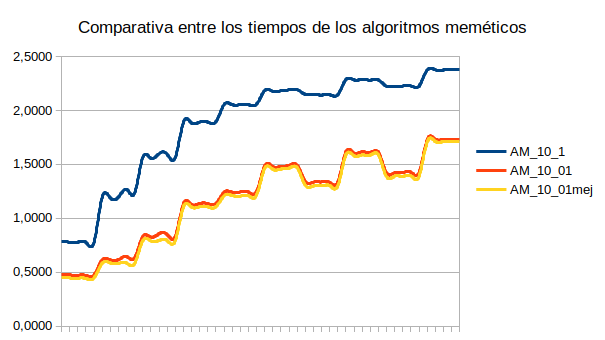
\includegraphics[width=0.65\textwidth]{data/tiempo_memeticos.png}
	\caption{Tiempo de ejecución por archivo en los algoritmos meméticos}
	\label{fig:tmemeticos}
\end{figure}

Ahora si nos fijamos en la gráfica \ref{fig:dispYT_mejores}, en la que podemos ver la dispersión y los tiempos de los mejores algoritmos de cada clase (genéticos y meméticos), es decir, el \textit{AM\_10\_01mej} y el \textit{AGG-uniforme}, se observa que a nivel de dispersión van bastante igualados, hay algunos tramos en los que el genético lleva menos dispersión y otros en los que más, pero por norma general, se solapan prácticamente en la totalidad del experimento. En cambio, en tiempo tenemos una superioridad clara del algoritmo genético, tardando este algo menos en ejecutarse que el memético.

Cabe destacar también los ``saltos'' que podemos observar en la dispersión. Si analizamos en qué archivos se aprecian esos saltos, nos daremos cuenta de que se trata de aquellos archivos en los que aumentamos $m$ pero mantenemos $n$, por ejemplo, cuando pasamos del archivo \textit{GKD-b\_25\_n100\_m10} al archivo \textit{GKD-b\_26\_n100\_m30}. Estas variaciones de $m$ son lo que produce los saltos que vemos en las gráficas respecto a la dispersión.

Aunque estos saltos se aprecien principalmente en la dispersión, también se puede ver en el tiempo de ejecución, aunque queda reflejado de una manera un tanto más sutil.

\begin{figure}[H]
    \centering
	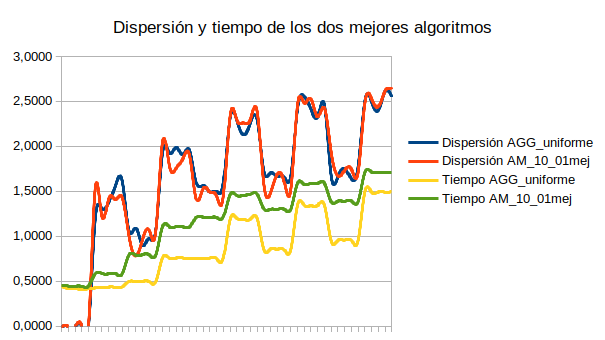
\includegraphics[width=0.65\textwidth]{data/dispYT_mejores.png}
	\caption{Dispersión y tiempo de los mejores algoritmos de cada tipo}
	\label{fig:dispYT_mejores}
\end{figure}

Por último, en la gráfica de la figura \ref{fig:tgeneticos} podemos ver los tiempos de ejecución por archivo de los algoritmos genéticos implementados.

Resulta curioso observar que los tiempos de ejecución de los modelos estacionarios son peores que los de los modelos generacionales, siendo este el resultado obtenido para ambos operadores de cruce.

Puesto que esto se da independientemente de los operadores de cruce, podemos concluir a partir de esta gráfica que \textbf{el operador de reemplazo del modelo estacionario resulta un tanto menos eficiente que el del modelo generacional}. Aunque esta diferencia en tiempo es minúscula, no deja de ser perceptible, por lo que debe de tratarse de un problema con el operador de reemplazo.

\begin{figure}[H]
    \centering
	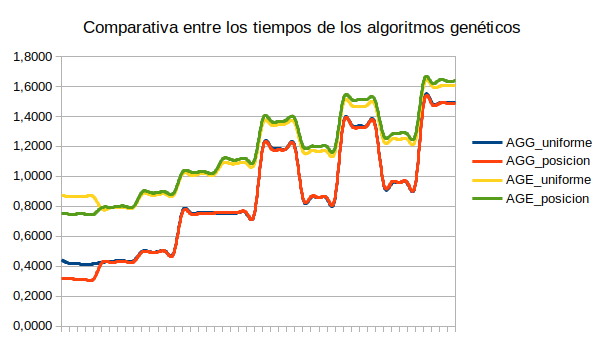
\includegraphics[width=0.65\textwidth]{data/tiempo_geneticos.png}
	\caption{Tiempo de ejecución por archivo en los algoritmos genéticos}
	\label{fig:tgeneticos}
\end{figure}

\newpage

\subsection{Conclusión general sobre los algoritmos estudiados}

Después de este estudio exhaustivo de los resultados obtenidos experimentalmente, sólo nos queda llegar a una conclusión.

Recapitulando, tenemos que los resultados obtenidos suelen ser mejores en los meméticos que en los genéticos, pero los tiempos de ejecución son algo mayores en estos últimos.

También tenemos que los modelos generacionales de algoritmos genéticos dan mejores resultados tanto en tiempo como en dispersión que los estacionarios.

Hemos concluido también que el operador de cruce uniforme es ligeramente superior al basado en posición, en base a los datos empíricos.

También podemos decir que el algoritmo de búsqueda local no queda descartado de una lista de posibles resoluciones a este problema, ya que tiene unos valores bastante aceptables, tanto en tiempo como en desviación, pudiendo dar algunos resultados incluso mejores que los genéticos o muy cercanos a estos.


Dicho esto, tenemos que los algoritmos meméticos proporcionan generalmente un resultado de mayor calidad que el resto, no obstante si el tiempo es un factor crítico, no sería problema optar por usar un algoritmo genético como sería \textit{AGG-uniforme} o, si los resultados no son críticos, una búsqueda local, que ya hemos visto que nos proporciona unos buenos resultados (aunque peor que los algoritmos implementados en esta práctica) y con un tiempo de ejecución bastante bueno en comparación con aquellos que nos proporcionan resultados de mayor calidad.









\end{document}